\documentclass[UTF8]{ctexart}
\usepackage{natbib}
\usepackage{capt-of}
\usepackage{graphicx}
\usepackage{multicol}
\usepackage{subfigure}
\usepackage{amsmath,amsthm}
\usepackage{amsfonts,amssymb}
\usepackage{listings}

\makeatletter

\makeatother

\begin{document}
\title{基于信息熵的中文词汇抽取和专有词汇(词组)词典构建 \\
\large{——方法、实现与实验}}


\author{计算机科学与技术\ 朱恬骅\ 09300240004}
\date{2012年11月}
\maketitle

\section{概述}
\subsection{本文目的}
由于中文的书写习惯不同于英语等西方语言,在英语语言学者中非常简单而普遍的词频统计方法应用于中文时需要首先完成对文本的分词。对中文文本进行分词成为进一步文本处理的先决条件。中文文本的分词准确程度将很大程度上影响后续分析的效果。

近年来,随着汉语学者在语言学和计算机科学方面的不断努力,各种新的分词算法正在向更高的分词准确率发起挑战。然而,由于计算机系统自身的局限,尽管在未登录词的识别方面也已得到可喜的成绩,各类分词算法都首先需要一个完备的词典和词频统计数据,以便得到较为准确的结果。

\subsection{当前研究概述}
\cite{Yamamoto:2001:USA:972778.972779} 提出了利用信息熵为无词语界限的语言(该文以日语为例)进行分词的思想。
\cite{GuSenProgrammer} 基于上述思想,给出了一个较为通俗的介绍,并且以人人网的用户产生的数据为例,展现了这一词汇抽取方法在应对新词和提示新热点的时候所展现出的能力。\cite{Feng:2004:AVC:1005380.1005384} 给出了一个更加清晰的用于中文文本词汇抽取的方法,其主要关注点在于字串的前驱和后继字符,并且主要展现了其在未登录词上的能力。

\subsection{本文方法和结构}
本文以\cite{GuSenProgrammer} 一文中提出的中文词汇的新词识别的基础上,实现了一个基于信息熵的中文词汇识别、抽取系统,并给出了此系统在识别财经新闻中专业词汇(词组)的一个应用,以演示该方法在处理以专业词汇为主的文本时所具备的优势。

在本文的实验部分,首先给出了这一词汇抽取系统在《人民日报》1998 年 1 月分词标注语料库上的表现,与人工分词的结果互为比较。实验表明,该方法在《人民日报》语料库上的词汇覆盖率为 64\% ,结合常用词表后覆盖率可以超过 96\% ;在所有找到的词汇中,正确率为 68\%~69\% ,这是因为系统缺少关于词组的知识,在词汇表中引入了较多的高频搭配所致。

在本文的应用部分,给出了这一系统在新浪网财经频道个股新闻板块 84.8万篇新闻中抽取出的词汇词频表,并介绍了利用这一词频表,结合分词算法进行词典迭代精化的方法及其结果。

最后,本文将给出一个利用矩阵分解模型进行词汇聚类和特征选择,从而进一步优化词典的简单示例。

\section{理论与方法}
\subsection{信源、信道和信息熵}
\cite{Shannon1948} 在 1948 年提出了信息熵的概念。他将信息熵定义为对不确定性的测量。熵的概念最早起源于物理学,用于度量一个热力学系统的无序程度。但在信息论中,熵越高,代表信道传输的信息量越大;熵越低,则意味着传输的信息越少。

\subsubsection{记忆性和马尔可夫性质}
任何能够产生符号的发送者都可以被认为是一个信道。信道的基本组成有其字母表$X$,字母表上的概率分布$P$。符号的接受者则被称为信宿。信道是信号(符号)传送的渠道\cite{RMEInformation}。 一个常用的信源模型是离散无记忆信源(discrete memoryless source,DMS)。DMS的定义如下所述。考虑一个信源$S$,在每单位时间中,从一个有限的集合$X = \{ X_1, X_2, \dots, X_N \}$(信源字母表)中独立地产生一个符号。由于集合有限且取值离散,我们称信源$S$是\textbf{离散}的。在$T$时间中,$S$产生的符号可用一个序列表示:$\{ x_1, x_2, \dots, x_T \}$。若这一过程中,事件$x_t = X_j$发生的概率与时间$t$无关,也与前一个符号$x_{t-1}$的取值无关。我们称这个信源$S$是\textbf{无记忆}(memoryless)的。满足上述两个特征的信源$S$即为\textbf{DMS}。相反地,如果符号$x_t$的取值与$x_{t-1}$有关,则该信道就是有记忆的。

为方便建模,这里再简单引入一下(一阶)马尔可夫性质(Markov property)的概念。马尔可夫性是指,一系列的随机变量$X_1, X_2, \dots $满足下列等式:

\begin{equation}
\Pr(X_{n+1}=x|X_1=x_1, X_2=x_2, \dots, X_n=x_n) = \Pr(X_{n+1} = x| X_n = x_n)
\end{equation}

亦即,$n$时刻信源所产生的符号仅与其前一个符号有关。类似地,我们可以定义2至$m$阶马尔可夫性质:

\begin{equation}
\begin{aligned}
&\Pr(X_n=x_n|X_{n-1}=x_{n-1}, X_{n-2}=x_{n-2}, \dots , X_1=x_1) \\
= &\Pr(X_n=x_n|X_{n-1}=x_{n-1}, X_{n-2}=x_{n-2}, \dots, X_{n-m}=x_{n-m})  \text{对于}n > m
\end{aligned}
\end{equation}

具有$m$阶马尔可夫性质的随机变量系列$X_1, X_2, \dots, X_N$称为$m$阶马尔可夫链(Markov chain)。显然地,我们可以通过恰当定义概率分布$\Pr(X_n=x_n|\dots)$,来使得高阶的马尔可夫链完成低阶的马尔可夫链的行为。尽管在实际中我们并不会这样做,在数学上,我们完全可以认为$m$阶马尔可夫链真包含$m-1$阶马尔可夫链。

\subsubsection{文本生成过程的信源建模}
\label{sec_generative_model}
在本文中,假设文本信息是由字母表为$X$的信源$S$所产生,其中$X$代表一个有限的现代汉语词汇的子集,$S$是一个DMS。在不引起混淆的情况下,我们用$P(X_i)$来表示上述式子。我们假设信道是无错的。本文所需要完成的工作即是通过观测$S$产生的符号序列$\mathcal{W}$来猜测$S$的字母表$X$和概率分布$P$。

将文本信息建模为DMS并非完全出于简化问题的需要,而是出于下面的考虑:其一,我们主要解决的是词频统计中的问题,而词频统计中并不关注词汇和词汇之间的顺序关系,采用所谓的“词袋”(bag-of-words)模型。其二,关于词汇的前后位置关系,即语法关系,应当由分词算法处理。而本文只关注如何对未分词的文本进行必要的词频统计处理,以利于分词算法发挥作用。如果在此越俎代庖,则会构成逻辑上依赖的循环。

然而在猜测的过程中,由于词汇的集合是待定的,信宿并没有获得完整的$X$。为了能够记录信源发来的信息,信宿采用的字母表是全体汉字的集合。对于发送来的词汇$W=c_1 c_2 c_3 \dots c_{n(W)}$,我们只能观测到它们的字符形式。借助于标点符号,我们将语料表示为一个句子的集合$\Gamma = \{ \gamma_1, \dots, \gamma_{N_s} \}$,其中每个句子都是一个字串$\gamma_i = \{ c_1, c_2, \dots, c_{N_s(i)} \}$,其中$c_i$是一个汉字。我们称之为在信宿视角下的信源$S$,记为$S'$。由于我们将抽象的层次从词汇下降到了字符,显然$S'$不再是一个DMS(例如,对于字串“力”,$p(\text{“力”}|\text{“巧克”})$的取值一定大于$p(\text{“力”}|\text{“上海”})$)。我们假设它具有$m$阶马尔可夫性,故字符集上的概率分布可以用$Pr(X_i=x_i|X_{i-1}=x_{i-1}, \dots, X_{i-m+1}=x_{i-m+1})$来表示。

\subsubsection{信息量和信息熵}

设 $X$ 是一个随机变量,其可能的取值范围为 $\{x_1, x_2, \dots, x_n\}$,$n < +\infty$,它们对应的概率分布为$p$。$X$的信息熵$H(X)$定义为:

\begin{equation}
H(X)=\text{E}(I(X))
\end{equation}

其中$I(X)$称为$X$的信息量,其定义如下:

\begin{equation}
I(X) = \sum_{i=1}^{n}{-p(x_i) \log_b{p(x_i)}}
\end{equation}

被求和项称为单个符号的信息量,用 $I(x_i)$ 表示。对数函数的基 $b$ 决定了信息量的单位,一般取为2,这时信息量的单位称比特(bit)。信源的信息熵就是信源概率函数的信息熵。

假设一个0-1 DMS,其信息熵函数的图像可见于图\ref{fig_entropy_function}。可见,两个符号的信息量函数是一个凸函数(concave),过高和过低的出现概率都会导致较低的函数值。这一特性可以被用于刻画信源发送符号时的丰富程度。

\begin{figure}
\center
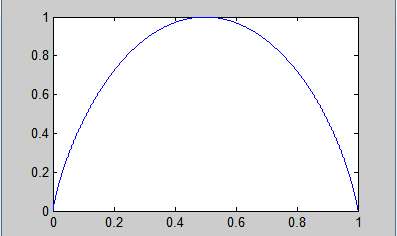
\includegraphics[width=0.6 \textwidth]{entropy_function.png}
\caption{0-1DMS的信息熵函数 H(x),横轴表示 $\Pr(X=1)$}
\label{fig_entropy_function}
\end{figure}

\subsection{对词汇的定义}
词汇是“语言中能独立运用的最小语法单位”。\cite{HuYushuXianHan} 它有两种主要特性:其一是“独立运用”,这是相对于语素这一概念而提出的。其二是“最小语法单位”,它决定了词汇的抽象层次是处在语法层面上的。由于本文不涉及对词汇的语义分析,这决定了词汇是目前所采取的抽象级别上所能处理的问题。

词汇之能够独立运用,主要体现在下述两种特性:其一,是外部的“自由程度”。这也同时体现了“最小单位”的两个方面。从“大到小”的方向上来看,“谢谢”是一个词而“谢谢你”不是一个词,因为前者参与句子构成时候可能的前后组合要比后者丰富。而从“很小到小”的方向上看,“中国银行”是一个专有名词,而“中国银”却不是词汇,尽管在一篇论述“中国银监会”和“中国银行”的文章中,“中国银”出现的次数比这两个专名的出现次数都要多,但它却不是自由的,因为它在给定的词汇表中只能作为前导的三个字出现。而“中国银行”则可作为名词参与句子,出现在不同的字词之后或之前。

其二是内部的“凝固性”。用\cite{GuSenProgrammer}中的例子,“电影院”是一个词而“的电影”不是一个词,是因为“电影院”的出现频率大于“电影”、“院”独立出现的频率之积,亦即假若信源$S'$在产生“电影院”这个字串的时候仅仅是出于随机而将它们拼凑在一起,这种情况的概率应当远小于“电影院”是由信源$S'$采用一条3阶马尔可夫链生成的情况。

\subsubsection{“自由程度”的衡量}
为了量化词语能够独立运用、自由参加句子组成的程度,我们引入上述信息熵的概念。令一个词$W$对应两个信源,一个是前导字串信源$S_W^L$,另一个是后继字串信源$S_W^R$。这两个信源的字母表皆为全体汉字的集合$C$,显然$C$是有限而离散的。在前文定义的基础上,我们定义信源$S_W^L$的概率分布为$\Pr(c_i) = freq(c_i W) \triangleq P_L(c_i)$,信源$S_W^R$的概率分布为$\Pr(c_i) = freq(W c_i) \triangleq P_R(c_i)$。显然,这两个信源都是DMS。由此,我们计算这两个信源的信息熵$H(S_W^L)$、$H(S_W^R)$。参考图\ref{fig_entropy_function},只有当$P_x (x=L, R)$的非零项平均分布时,其信息熵才能取得最大值。任何偏离平均分布的情况下都会导致信息熵函数值减小。因而,我们可以用信息熵函数的这种性质定义字串的前导/后继自由度。

考虑到词根(定位语素)的存在,一个字串是词,只有当它前导和后继的自由度都很大的时候才能被认为是词。我们据此定义字串的自由度$free(W)$为:

\begin{equation}
free(W) = \min \{ H(S_W^L), H(S_W^R) \}
\label{eqn_def_free}
\end{equation}

\subsubsection{“凝固程度”的衡量}
为了用统计的方法能够衡量词汇内在的凝固性,我们考虑\ref{sec_generative_model}中定义的信源$S$。假设字串$W=c_1 c_2 c_3 \dots c_n$是一个词汇,显然有
\begin{equation}
\hat{p}(W) = \max\limits_{a}\prod\limits_{i=1}^{\|a\|-1} (freq(c_{a_i} c_{a_i+1} \dots c_{a_{i+1}-1})) \ll freq(W) 
\end{equation}
其中$a$是对数列$\{1,2,3,\dots,n\}$的一个\textbf{划分},函数$freq(W)$表示一个字串$W$在观测到的符号串中出现的频率。因此,我们定义字串$S$的凝固度$coh(W)$为:

\begin{equation}
coh(W) = \frac{freq(W)}{\hat{p}(W)}
\label{eqn_def_coh}
\end{equation}

\subsubsection{对词汇的定义}
我们引入三个参数$\theta_f$,$\theta_c$和$m$。其中$m$是信源$S'$所满足的马尔可夫性质的最大阶数,亦即词的最大长度。$\theta_f < free(W)$且$\theta_c < coh(W)$时,字串$W$才能够被认为可能是一个词。

\subsection{实现方法}


\section{实验}
\subsection{《人民日报》1998年1月标注语料库上的实验}
\paragraph{检测范围} 采用的是《人民日报》1998年1月标注语料库。只检测长度介于2至5(含)之间,在语料库中出现次数大于等于10的词汇。参数选择为:$\theta_c = 100, \theta_f = 1.0, m = 5$。
\paragraph{检测结果} 本文的方法检测出候选字串6577个,人工标注的结果为7015个。其中:相同词汇有4457个,占本文方法检出词汇的(覆盖率)67.7\%;未检出词汇2558个,占词汇总个数的36.5\%,正确率为63.5\%。
\paragraph{结果讨论} 除去相当数量的错误结果外,有必要说明人工标注规则和自动抽取规则中的显著不同。在人工标注规则中,姓名被分割为两个词,由多个通用或专有名词组成的专有名词被分割为多个通用名词,并在最外部加括号以示为准确。如此,“江泽民”在自动抽取时被认为是一个词,而在手工标注时则不是;“中国共产党”在自动抽取时被认定为一个词,而在手工标注中则为“[中国/共产党]”。同时,由于《人民日报》语体的特殊性,在结果中会出现大量满足长度限制的固定搭配,这些固定搭配中的词并未能够在给定的语料中体现出其独立性,而手工标注由于了解这方面的先验知识,所以能够作出正确的判断。例子有:“由公安机关”、“本报评论员”、“五个一工程”、“级偏北风”等。

一方面,我们需要通过归并词组中的词语来减少词典的大小;另外一方面,寻找到的词组也可能会有益于我们减少数据的维度。例如,将人名视作单个词语,就有助于我们更好地识别语篇句的主题;将套话、固定格式的短语视作词汇,有助于我们方便地去除噪音,对文本进行降维以利后续的处理。这一点将在处理财经文本信息时进行讨论。

\paragraph{对词组的二次切分} 为减少上述问题带来的问题,对于长度超过3的字串,程序进行迭代切分,每次迭代中检查词典中现存的字串,如果分拆成两个部分时二者皆已存在于词典中,或一者存在于词典而另一者长度为1,则进行切分并删除原先的词组。进行上述操作后的结果如下。
\begin{table}\centering
\caption{进行词组二次切分后的结果}
\label{tab_divide_phrase}
\begin{tabular}{r|cccccc}
迭代次数 & 0 & 1 & 2 & 3 & 4 & 5 \\
本文方法所得字串数 & 6577 & 6464 & 6131 & 6065 & 6042 & 6042\\
标准(人工)词汇数 & 7015 & 7015 & 7015 & 7015 & 7015 & 7015\\
相同词汇数量 & 4457 & 4317 & 4219 & 4171 & 4163 & 4163\\
覆盖率 & 0.6353 & 0.6154 & 0.6014 & 0.5946 & 0.5934 & 0.5934\\
正确率 & 0.6776 & 0.6678 & 0.6881 & 0.6877 & 0.6890 & 0.6890\\
\end{tabular}
\end{table}

可以看出,这种迭代的方法并不能有效提高正确率,并且较大幅度地牺牲了覆盖率。这说明,本方法必须引入少量的先验知识(即常用词的项目)参与词频统计。通过引入1000个高频词(据\cite{ChangyongCibiaoCaoan}),正确率提高到95.8\%,覆盖率为66.8\%。但是这种方法并不能从根本上改善算法的运行效果。

\subsection{参数选择}
上述参数选择中$\theta_c$和$\theta_f$有相当的随意性。为选择一个较好的参数,进行了更加具体的实验。

首先我们保持$\theta_c=100$不变,更改$\theta_f$的值,覆盖率和正确率随$\theta_f$的变化如图\ref{fig_theta_f}所示。

\begin{figure}
\center
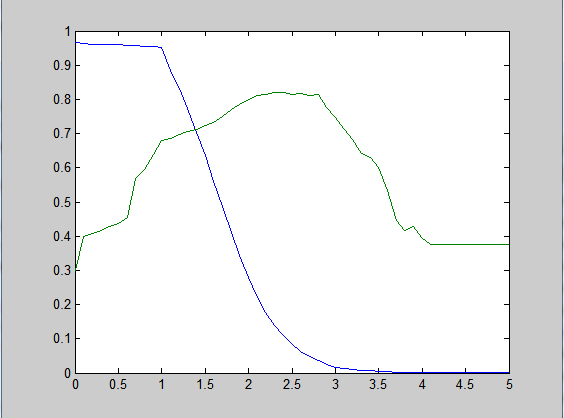
\includegraphics[width=0.8 \textwidth]{theta_f_percent.png}
\caption{覆盖率和正确率随$\theta_f$的变化}
\label{fig_theta_f}
\end{figure}

图中,蓝色表示覆盖率,绿色表示正确率。图\ref{fig_theta_c}展示了二者随$\theta_c$变化的曲线。

\begin{figure}
\center
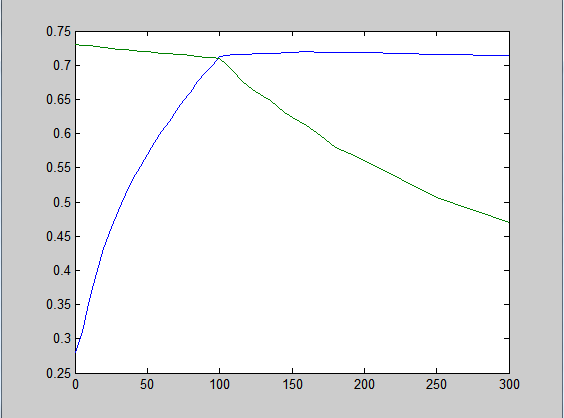
\includegraphics[width=0.8 \textwidth]{theta_c_percent.png}
\caption{覆盖率和正确率随$\theta_c$的变化}
\label{fig_theta_c}
\end{figure}




\section{讨论}


\bibliographystyle{newapa}
\bibliography{cnlp}

\end{document}